\documentclass{standalone}
\usepackage{pgfplots}
\pgfplotsset{compat=1.17}

\begin{document}

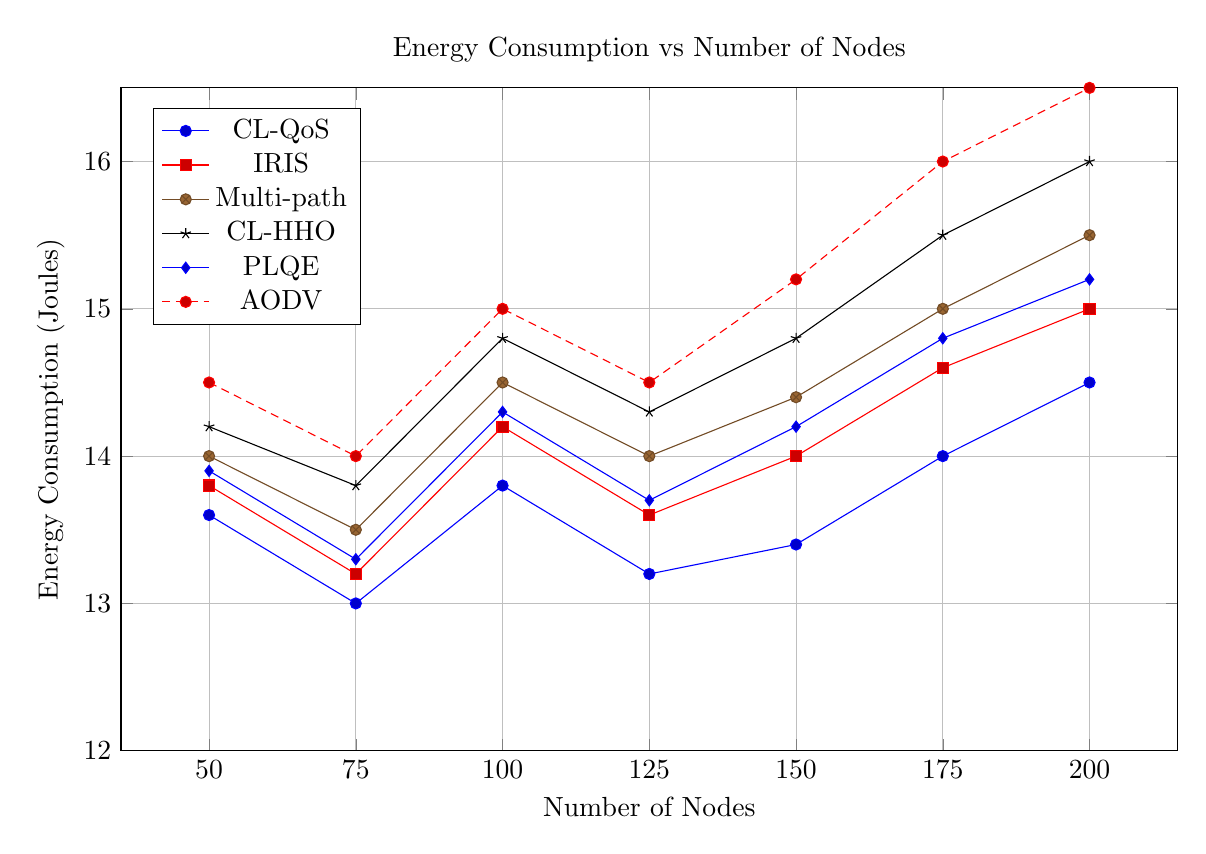
\begin{tikzpicture}

\begin{axis}[
width=15cm,
height=10cm,
title={Energy Consumption vs Number of Nodes},
xlabel={Number of Nodes},
ylabel={Energy Consumption (Joules)},
ymin=12, ymax=16.5,
xtick={50,75,100,125,150,175,200},
ytick={12,13,14,15,16},
legend pos=north west,
grid=both
]

\addplot coordinates {(50,13.6) (75,13.0) (100,13.8) (125,13.2) (150,13.4) (175,14.0) (200,14.5)};
\addplot coordinates {(50,13.8) (75,13.2) (100,14.2) (125,13.6) (150,14.0) (175,14.6) (200,15.0)};
\addplot coordinates {(50,14.0) (75,13.5) (100,14.5) (125,14.0) (150,14.4) (175,15.0) (200,15.5)};
\addplot coordinates {(50,14.2) (75,13.8) (100,14.8) (125,14.3) (150,14.8) (175,15.5) (200,16.0)};
\addplot coordinates {(50,13.9) (75,13.3) (100,14.3) (125,13.7) (150,14.2) (175,14.8) (200,15.2)};
\addplot coordinates {(50,14.5) (75,14.0) (100,15.0) (125,14.5) (150,15.2) (175,16.0) (200,16.5)};

\legend{CL-QoS, IRIS, Multi-path, CL-HHO, PLQE, AODV}

\end{axis}

\end{tikzpicture}

\end{document}